% This file was created with tikzplotlib v0.10.1.post9.
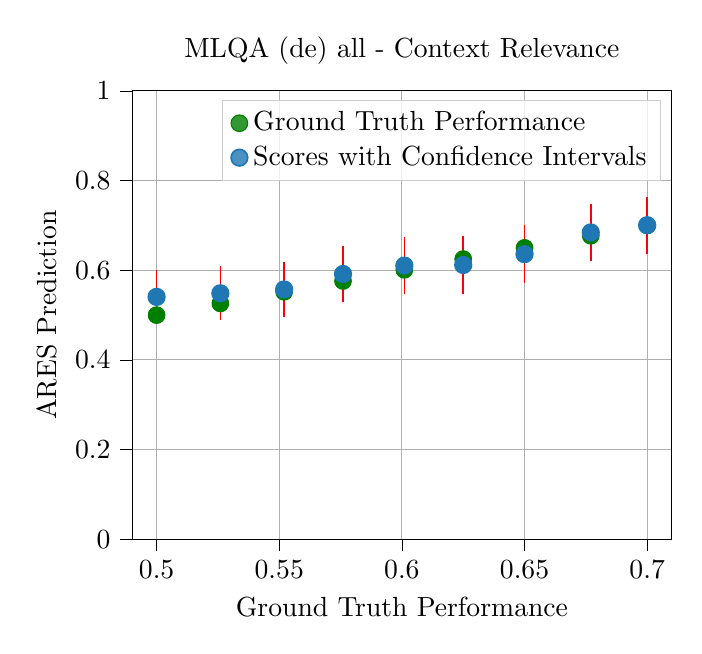
\begin{tikzpicture}

\definecolor{darkgrey176}{RGB}{176,176,176}
\definecolor{green01270}{RGB}{0,127,0}
\definecolor{lightgrey204}{RGB}{204,204,204}
\definecolor{steelblue31119180}{RGB}{31,119,180}

\begin{axis}[
legend cell align={left},
legend style={
  fill opacity=0.8,
  draw opacity=1,
  text opacity=1,
  draw=lightgrey204,
  mark options={mark size=3}
},
tick align=outside,
tick pos=left,
title={MLQA (de) all - Context Relevance},
x grid style={darkgrey176},
xlabel={Ground Truth Performance},
xmajorgrids,
xmin=0.49, xmax=0.71,
xtick style={color=black},
y grid style={darkgrey176},
ylabel={ARES Prediction},
ymajorgrids,
ymin=0, ymax=1,
ytick style={color=black}
]
\addplot [draw=green01270, fill=green01270, mark size=3pt, mark=*, only marks]
table{%
x  y
0.5 0.5
0.526 0.526
0.552 0.552
0.576 0.576
0.601 0.601
0.625 0.625
0.65 0.65
0.677 0.677
0.7 0.7
};
\addlegendentry{Ground Truth Performance}
\path [draw=red, semithick]
(axis cs:0.5,0.481)
--(axis cs:0.5,0.601);

\path [draw=red, semithick]
(axis cs:0.526,0.488)
--(axis cs:0.526,0.61);

\path [draw=red, semithick]
(axis cs:0.552,0.495)
--(axis cs:0.552,0.619);

\path [draw=red, semithick]
(axis cs:0.576,0.529)
--(axis cs:0.576,0.654);

\path [draw=red, semithick]
(axis cs:0.601,0.547)
--(axis cs:0.601,0.674);

\path [draw=red, semithick]
(axis cs:0.625,0.548)
--(axis cs:0.625,0.676);

\path [draw=red, semithick]
(axis cs:0.65,0.572)
--(axis cs:0.65,0.7);

\path [draw=red, semithick]
(axis cs:0.677,0.621)
--(axis cs:0.677,0.748);

\path [draw=red, semithick]
(axis cs:0.7,0.637)
--(axis cs:0.7,0.764);

\addplot [semithick, steelblue31119180, mark=*, mark size=3, mark options={solid}, only marks]
table {%
0.5 0.540622710622711
0.526 0.54868978805395
0.552 0.557272727272727
0.576 0.591603375527426
0.601 0.610528052805281
0.625 0.611786941580756
0.65 0.635952380952381
0.677 0.684399008674102
0.7 0.700512820512821
};
\addlegendentry{Scores with Confidence Intervals}
\end{axis}

\end{tikzpicture}
